\achapter{17}{Compact Spaces}\label{chap:Compact_topology}


\vspace*{-17 pt}
\framebox{
\parbox{\dimexpr\linewidth-3\fboxsep-3\fboxrule}
{\begin{fqs}
\item What is a cover of a subset of a topological space? What is an open cover?
\item What is a subcover of a cover?
\item What is a compact subset of a topological space?
\item What is one application of compactness?
\item How do we characterize the compact subsets of $\R^n$? What theorem provides this characterization? 
\end{fqs}}}

\vspace*{13 pt}

\csection{Introduction}\label{sec_compact_top_intro}

Closed and bounded intervals have important properties in calculus. Recall, for example, that every real-valued function that is continuous on a closed interval $[a, b]$ attains a maximum and minimum value on that interval. The question we want to address in this section is if there is a corresponding characterization for subsets of topological spaces that ensure that continuous real-valued functions with domains in topological spaces attain maximum and minimum values. The property that we will develop is called compactness.

The word ``compact" might bring to mind a notion of smallness, but we need to be careful with the term. We might think that the interval $(0, 0.5)$ is small, but $(0, 0.5)$ is homeomorphic to $\R$, which is not small. Similarly, we might think that the interval $[-10000, 10000]$ is large, but this interval is homeomorphic to the ``small" interval $[-0.00001, 0.000001]$. As a result, the concept of compactness does not correspond to size, but rather structure, in a way. We will expand on this idea in this section. 

Since a topology defines open sets, topological properties are often defined in terms of open sets. Let us consider an example to see if we can tease out some of the details we will need to get a useful notion of compactness. Consider the open interval $(0, 1)$ in $\R$. Suppose we write $(0, 1)$ as a union of open balls. For example, let $O_n = \left(\frac{1}{n}, 1-\frac{1}{n}\right)$ for $n \in \Z^+$ and $n \geq 3$. Notice that $(0, 1) \subseteq \bigcup_{n \geq 3} O_n$. Any collection of open sets whose union contains $(0, 1)$ is called an \emph{open cover} of $(0, 1)$. Working with a larger number of sets is generally more complicated than working with a smaller number, so it is reasonable to ask if we can reduce the number of sets in our open cover of $(0, 1)$ and still cover $(0, 1)$. In particular, working with a finite collection of sets is preferable to working with an infinite number of sets (we can exhaustively check all of the possibilities in a finite setting if necessary). Notice that $O_n \subset O_{n+1}$ for each $n$, so we can eliminate many of the sets in this cover. However, if we eliminate enough sets so that we are left with only finitely many, then there will be a maximum value of $n$ so that $O_n$ remains in our collection. But then $\frac{1}{2n}$ will not be in the union of our remaining collection of sets. As a result, we cannot find a finite collection of the $O_n$ whose union contains $(0, 1)$. Note that there may be some collections of open sets that cover of $(0,1)$ for which there is a finite subcollection of sets that also cover $(0,1)$. For example, if we let $U_n = \left(n-\frac{3}{4}, n+\frac{3}{4}\right)$, then $(0,1) \subseteq \bigcup_{n \in \Z} U_n$, and $(0,1) \subseteq U_{0} \cup U_1$. The main point is that there is at least one collection of open sets that covers $(0,1)$ for which there is no finite subcollection of sets that covers $(0,1)$. 
 
Let's apply the same idea now to the set $[0, 1]$. Suppose we extend our open cover $\{O_n\}$ to be an open cover of the closed interval $[0, 1]$ by including two additional open balls in $\R$: $O_0 = B(0, 0.5)$ and $O_1 = B(1, 0.5)$. Now the sets $O_0$, $O_1$, and $O_4$ form a finite collection of sets that covers $[0, 1]$. So even though the interval $[0, 1]$ is ``larger" than $(0, 1)$ in the sense that $(0, 1) \subset [0, 1]$ we can represent $[0, 1]$ in a more efficient (that is finite) way in terms of open sets than we can the interval $(0, 1)$. This is the basic idea behind compactness. 

\begin{definition} \label{def:compact} A subset $A$ of a topological space $X$ is \textbf{compact}\index{compact subset} if for every set $I$ and \emph{every} family of open sets $\{O_{\alpha}\}$ with $\alpha \in I$ such that $A \subseteq \bigcup_{\alpha \in I} O_{\alpha}$, there exists a finite subfamily $\{O_{\alpha_1}, O_{\alpha_2}, \ldots, O_{\alpha_n}\}$ such that $A \subseteq \bigcup_{i = 1}^n O_{\alpha_i}$. 
\end{definition}

If $(X,\tau)$ is a topological space and $X$ is a compact subset of $X$, then we say that $X$ is a \emph{compact topological space}. There is some terminology associated with Definition \ref{def:compact}.

\begin{definition} A \textbf{cover}\index{cover} of a subset $A$ of a topological space $X$ is a collection $\{S_{\alpha}\}$  of subsets of $X$ for $\alpha$ in some indexing set $I$ so that $A \subseteq \bigcup_{\alpha \in I} S_{\alpha}$. In addition, if each set $S_{\alpha}$ is an open set, then the collection $\{S_{\alpha}\}$ is an \textbf{open cover}\index{cover!open} for $A$.
\end{definition}

\begin{definition} A \textbf{subcover}\index{subcover} of a cover $\{S_{\alpha}\}_{\alpha \in I}$ of a subset $A$ of a topological space $X$ is a collection $\{S_{\beta}\}$ for $\beta \in J$, where $J$ is a subset of $I$ such that $A \subseteq \bigcup_{\beta \in J} S_{\beta}$. In addition, if $J$ is a finite set, the subcover $\{S_{\beta}\}_{\beta \in J}$ is a \textbf{finite subcover}\index{subcover!finite} of $\{S_{\alpha}\}_{\alpha \in I}$.
\end{definition}

So the sets $O_0$, $O_1$, and $O_4$ in our previous example form a finite subcover of the open cover $\{O_n\}_{n \geq 3}$. 

Using the terminology we have now established, we can restate the definition of compactness in the following way: a subset $A$ of a topological space $X$ is compact if every open cover of $A$ has a finite subcover of $A$.

\begin{pa} Determine if the subset $A$ of the topological space $X$ is compact. Either prove $A$ is compact by starting with an arbitrary infinite cover and demonstrating that there is a finite subcover, or find a specific infinite cover and prove that there is no finite subcover.
\be
\item $A = \{-2, 3, e, \pi, 456875\}$ in $X = \R$ with the Euclidean topology. Generalize this example.

\item $A = (0, 1]$ in $X = \R$ with the Euclidean topology.

\item $A = \left\{\frac{1}{n} \mid n \in \Z^+\right\}$ in $X = \R$ with the Euclidean topology.

\item $A = \Z^+$ in $X = \R$ with the Euclidean topology.

\item $A = \Z^+$ in $X = \R$ with the finite complement topology.

\item $A = \R$ in $X = \R$ with the Euclidean topology.

\ee

\end{pa}

\begin{comment}

\ActivitySolution

\be
\item  Let $X$ be a topological space and let $A$ be a finite subset of $X$. We will demonstrate that $A$ is compact. Suppose $\CC = \{O_{\alpha}\}_{\alpha \in I}$ is an open cover of $A$ with indexing set $I$. For each $a \in A$, let $O_a$ be an element of $\CC$ with $a \in O_a$. Then $\{O_a\}_{a \in A}$ is a finite subset of $\CC$ that covers $A$.

\item  For each $n \in Z^+$, let $O_n = \left(\frac{1}{n}, 1+\frac{1}{n}\right)$. Then $\CC = \{O_n\}_{n \in \Z^+}$ is an open cover of $A$. To show that $\CC$ contains no finite subcover of $A$, proceed by contradiction and assume that there is a positive integer $k$ and a finite collection $U_1$, $U_2$, $\ldots$, $U_k$ of sets in $\CC$ such that $A \subseteq \cup_{i=1}^k U_i$. For each $i$ let $U_i = (a_i, b_i)$, and let $m = \min\{a_i \ \mid| \ 1 \leq i \leq k\}$. Then $\frac{1}{2a_m}$ is in $A$, but not in $\cup_{i=1}^k U_i$. So $\CC$ contains no finite subcover of $A$ and $A$ is not compact.

\item  The set $A$ is not compact, with an argument just like the one in part 2.

\item  The set A is not compact. For each $n \in \Z^+$, let $O_n = \left(n-\frac{1}{2}, n+\frac{1}{2} \right)$. Then $\CC = \{O_n\}_{n \in \Z^+}$ is an open cover of $\Z^+$. If $n \in Z^+$ and we remove the set $O_n$ from the collection $\CC$, then the union of the remaining sets in $\CC$ will not contain $n$. So $\CC$ contains no finite cover of $A$.

\item  We show that $A$ is compact. Let $\CC = \{O_{\alpha}\}_{\alpha \in I}$ be an open cover of $A$ with indexing set $I$. Choose an $\alpha \in I$ and let $U_0 = O_{\alpha}$. We know that $\R \setminus U_0$ is finite. Let $\{x_1, x_2, \ldots, x_k\} = \R \setminus U_0$. For each $i$ there is a set $U_i$ in $\CC$ such that $x_i \in U_i$. Then $A \subseteq \R = \cup_{i=0}^k U_i$ and so $\CC$ contains a finite subcover of $A$. Therefore, $A$ is compact. This argument shows that any nonempty subset of any space with the finite complement topology is compact.

\item  The set $\R$ is not compact. Let $x \in \R$ and let $O_x = (-x, x)$ (with $O_0 = \emptyset$). Then $\CC = \{O_x\}_{x \in \R}$ is an open cover of $\R$. If $\CC$ contains a finite subcover $\{U_i\}_{1 \leq i \leq k}$ with $U_i = (-x_i, x_i)$, then the set $\{x_i\}_{1 \leq i \leq k}$ has an upper bound $M$. But then $M + 1$ is not in $\cup_{1 \leq i \leq k} U_i$. So $\CC$ contains no finite subcover of $\R$ and $\R$ is not compact.

\ee

\end{comment}
There are two perspectives by which we can look at compactness. If $(X,\tau_X)$ is a topological space and $A$ is a subset of $X$, then Definition \ref{def:compact} tells us what it means for $A$ to be compact as a subset of $X$. From this perspective, we use open sets in $X$ to make open covers of $A$. We can also consider $A$ as a subspace of $X$ using the subspace topology $\tau_A$. From this perspective we can examine the compactness of $A$ using relatively open sets for open covers. Exercise (\ref{ex:subspace_compact}) tells us that these two perspectives are equivalent, so we will use whatever perspective is appropriate for a given situation. 


\csection{Compactness and Continuity}\label{sec_compact_cont}

In our preview activity we learned about compactness -- the analog of closed intervals from $\R$ in topological spaces. Recall that a subset $A$ of a topological space $X$ is compact if every open cover of $A$ has a finite sub-cover. As we will see, the definition of compactness is exactly what we need to ensure results of the type that continuous real-valued functions with domains in topological spaces attain maximum and minimum values on compact sets. 

We might expect that compact sets have certain properties, but we must be careful which ones we assume.

\begin{activity} \label{act:compact_clopen} Let $X = \{a,b,c,d\}$ and give $X$ the topology $\tau = \{\emptyset, \{a\}, \{b,c\}, \{a,b,c\}, X\}$. 
\ba
\item Explain why every finite subset of a topological space must be compact. 

\item Find, if possible, a subset of $X$ that is compact and open. If no such subset exists, explain why.

\item If $A$ is a compact subset of $X$, must $A$ be open? Explain.

\item Find, if possible, a subset of $X$ that is compact and closed. If no such subset exists, explain why.

\item If $A$ is a compact subset of $X$, must $A$ be closed? Explain.

\ea

\end{activity}

\begin{comment}

\ActivitySolution

\ba
\item Suppose that $X$ is a topological space and $A = \{a_1, a_2, \ldots, a_n\}$ is a finite subset of $X$. If $\mathcal{O} = \{O_{\alpha}\}_{\alpha \in I}$ is an open cover of $A$, then for each $1 \leq k \leq n$ there is an $\alpha_k$ such that $a_k \in O_{\alpha_k}$. So $\{O_{\alpha_k}\}_{1 \leq k \leq n}$ is a finite subcover of $\mathcal{O}$. So every finite subset of a topological space is compact. 

\item The set $\{a\}$ is both open and compact in $X$.

\item The set $\{c\}$ is compact but not open in $X$.

\item The set $\{d\}$ is closed and compact in $X$.

\item The set $\{a\}$ is compact, but not closed because $\{a\}^c$ is not open. 


\ea

\end{comment}


The message of Activity \ref{act:compact_clopen} is that compactness by itself is not related to closed or open sets. We will see later, though, that in some reasonable circumstances, compact sets and closed sets are related. For the moment, we take a short detour and ask if compactness is a topological property. 

\begin{activity} \label{act:compact_invariant} Let $(X, \tau_X)$ and $(Y, \tau_Y)$ be topological spaces, and let $f: X \to Y$ be continuous. Assume that $A$ is a compact subset of $X$. In this activity we want to determine if $f(A)$ must be a compact subset of $Y$. 
\ba 
\item What do we need to show to prove that $f(A)$ is a compact subset of $Y$? Where do we start?

\item If we have an open cover of $f(A)$ in $Y$, how can we find an open cover $\{U_{\alpha}\}$ for $A$? Be sure to verify that what you claim is actually an open cover of $A$. 

\item What do we know about any open cover of $A$? 

\item Complete the proof of the following theorem.

\begin{theorem} Let $(X, \tau_X)$ and $(Y, \tau_Y)$ be topological spaces, and let $f: X \to Y$ be continuous. If $A$ is a compact subset of $X$, then $f(A)$ is a compact subset of $Y$. 
\end{theorem}

\ea

\end{activity}

\begin{comment}

\ActivitySolution

\ba 
\item To prove that $f(A)$ is a compact subset of $Y$, let $\{O_{\alpha}\}$ be a collection of open subsets of $Y$ for $\alpha$ in some indexing set $I$ such that $f(A) \subseteq \bigcup_{\alpha \in I} O_{\alpha}$. We will show that there is a positive integer $n$ and a finite collection $O_{\alpha_1}$, $O_{\alpha_2}$, $\ldots$, $O_{\alpha_n}$, of sets in $\{O_{\alpha}\}_{\alpha \in I}$ that cover $f(A)$. 

\item Since $f$ is continuous, the sets $U_{\alpha} = f^{-1}(O_{\alpha})$ are open in $X$ for each $\alpha \in I$. Also, if $a \in A$, then $f(a) \in \bigcup_{\alpha \in I} O_{\alpha}$. So $f(a) \in O_{\beta}$ for some $\beta \in I$. Then $a \in f^{-1}(O_{\beta}) = U_{\beta} \subseteq \bigcup_{\alpha \in I} U_{\alpha}$. So $A \subseteq \bigcup_{\alpha \in I} U_{\alpha}$. Thus, the sets $U_{\alpha}$ for $\alpha \in I$ form an open cover of $A$.

\item The fact that $A$ is compact means that there is a positive integer $n$ and a finite collection $U_{\alpha_1}$, $U_{\alpha_2}$, $\ldots$, $U_{\alpha_n}$, of sets in $\{U_{\alpha}\}_{\alpha \in I}$ that cover $A$.

\item We will prove that $f(A) \subseteq \bigcup_{i=1}^n O_{\alpha_i}$, which will complete our proof that every open cover of  $f(A)$ in $Y$ has a finite sub-cover. 

Let $b \in f(A)$. Then $f^{-1}(b) \in A \subseteq \bigcup_{i=1}^n U_{\alpha_i}$. It follows that $f^{-1}(b) \in U_{\alpha_i}$ for some $1 \leq i \leq n$. Then $b \in f\left(U_{\alpha_i}\right) \subseteq O_{\alpha_i}$. Therefore, 
\[f(A) \subseteq \bigcup_{i=1}^n O_{\alpha_i}.\]
This verifies that every open cover of $f(A)$ has a finite subcover.  

\ea

\end{comment}

A consequence of Activity \ref{act:compact_invariant} is that compactness is a topological property. 

\begin{corollary} Let $(X, \tau_X)$ and $(Y, \tau_Y)$ be homeomorphic topological spaces. Then a subset $A$ of $X$ is compact if and only if $f(A)$ is compact in $Y$. 
\end{corollary}

\csection{Compact Subsets of $\R^n$}\label{sec_compact_rn}

The metric space $(\R^n,d_E)$ is not compact since the open cover $\{B(0, n)\}_{n \in \Z^+}$ has no finite sub-cover.  Since we have already shown that $(\R,d_E)$ is homeomorphic to the topological subspaces $(a,b)$, $(-\infty, b)$, and $(a,\infty)$ for any $a, b \in \R$, we conclude that no open intervals are compact. Similarly, no half-closed intervals are compact. In fact, we will demonstrate in this section that the compact subsets of $(\R^n, d_E)$ are exactly the subsets that are closed and bounded. The first step is contained in the next activity.

\begin{activity} \label{act:metric_compact_closed} We have seen that compact sets can be either open or closed. However, in certain situations compact sets must be closed. We investigate that idea in this activity. Let $A$ be a compact subset of a Hausdorff topological space $X$. We will examine why $A$ must be a closed set.
\ba
\item To prove that $A$ is a closed set, we consider the set $X \setminus A$. What property of $X \setminus A$ will ensure that $A$ is closed? How do we prove that $X \setminus A$ has this property?

\item Let $x \in X \setminus A$. Assume that $A$ is a nonempty set (why can we make this assumption)? For each $a \in A$, why must there exist disjoint open sets $O_{xa}$ and $O_a$ with $x \in O_{xa}$ and $a \in O_a$? 

\item Why must there exist a positive integer $n$ and elements $a_1$, $a_2$, $\ldots$, $a_n$ in $A$ such that the sets $O_{a_1}$, $O_{a_2}$, $\ldots$, $O_{a_n}$ form an open cover of $A$?

\item Now find an open subset of $X \setminus A$ that has $x$ as an element. What does this tell us about $A$?

\ea

\end{activity}

\begin{comment}

\ActivitySolution

\ba
\item To show that $A$ is closed, we need to show that $X \setminus A$ is open. To show that $X \setminus A$ is open, we can demonstrate that $X \setminus A$ is a neighborhood of each of its points.

\item Since $\emptyset$ is always closed, if $A = \emptyset$ we are done. So we can assume that $A \neq \emptyset$. Let $x \in X \setminus A$. Since $X$ is Hausdorff, we can separate points by disjoint open sets. So for each $a \in A$, there exist disjoint open sets $O_{xa}$ and $O_a$ with $x \in O_{xa}$ and $a \in O_a$. 

\item The collection $\{O_a \mid a \in A\}$ is an open cover of $A$. The fact that $A$ is compact means that there is a finite subcover for this cover. That is, there exist a positive integer $n$ and elements $a_1$, $a_2$, $\ldots$, $a_n$ in $A$ such that the sets $O_{a_1}$, $O_{a_2}$, $\ldots$, $O_{a_n}$ form an open cover of $A$.

\item Let $O = \bigcap_{k=1}^n O_{xa_k}$. Note that if $a \in A$, then $a \in O_{a_k}$ for some $k$. But $O_{xa_k} \cap O_{a_k} = \emptyset$, so $a \notin O_{xa_k}$. Since $O \subseteq O_{xa_k}$, it is the case that $a \notin O$. Thus, $O \cap A = \emptyset$ and $O \subseteq X \setminus A$. We know that $x \in O_{xa_k}$ for every $k$, so $x \in O$. A finite union of open sets is open, so $O$ is open. This means that $X \setminus A$ is a neighborhood of each of its points and is therefore open. So $A$ is closed. 

\ea

\end{comment}


The result of Activity \ref{act:metric_compact_closed} is summarized in Theorem \ref{thm:metric_compact_closed}.

\begin{theorem} \label{thm:metric_compact_closed} If $A$ is a compact subset of a Hausdorff topological space, then $A$ is closed. 
\end{theorem}

Theorem \ref{thm:metric_compact_closed} tells us something about compact subsets of $(\R^n, d_E)$. Since every metric space is Hausdorff, we can conclude the following corollary.

\begin{corollary} If $A$ is a compact subset of $(\R^n, d_E)$, then $A$ is closed.
\end{corollary}


To classify the compact subsets of $(\R^n, d_E)$ as closed and bounded, we need to discuss what it means for a set in $\R^n$ to be bounded. The basic idea is straightforward -- a subset of $\R^n$ is bounded if it doesn't go off to infinity in any direction. In other words, a subset $A$ of $\R^n$ is bounded if we can construct a box in $\R^n$ that is large enough to contain it. Thus, the following definition.

\begin{definition} \label{def:n_cube} A subset $A$ of $\R^n$ is \textbf{bounded}\index{bounded subset of $\R^n$} if there exists $M > 0$ such that $A \subseteq Q^n_M$, where 
\[Q^n_M = \{(x_1,x_2, \ldots, x_n) \mid -M \leq x_i \leq M \text{ for every } 1 \leq i \leq n\}.\]
\end{definition}

The set $Q^n_M$ in Definition \ref{def:n_cube} is called the \emph{standard} $n$\emph{-dimensional cube of size M}.  A standard 3-dimensional cube of size $M$ is shown in Figure \ref{F:M_cube}.
\begin{figure}[h]
\begin{center}
\resizebox{!}{1.5in}{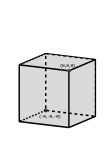
\includegraphics[trim=0.65cm 0.7cm 0.55cm 1.85cm, clip]{M_cube.png}} 
\caption{A standard 3-cube $Q^3_M$.} 
\label{F:M_cube}
\end{center}
\end{figure}
%\includegraphics[trim=left bottom right top, clip]{file}


An important fact about standard $n$-cubes is that they are compact subsets of $\R^n$. Compactness is a complicated property -- it is difficult to prove a result that is true about every open cover. As a result, the proof of Theorem \ref{thm:Compact_cubes} is quite technical, but it is a critical step to classifying the compact subsets of $\R^n$. 

\begin{theorem} \label{thm:Compact_cubes} Let $n \in \Z^+$. The standard $n$-dimensional cube of size $M$ is a compact subset of $\R^n$ for any $M > 0$. 
\end{theorem}

\begin{proof} We proceed by contradiction and assume that there is an $n \in \Z^+$ and a positive real number $M$ such that $Q^n_M$ is not compact. So there exists an open cover $\{O_{\alpha}\}$ with $\alpha$ in some indexing set $I$ of $Q^n_M$ that has no finite sub-cover. Let $Q_0 =  Q^n_M$ so that $Q_0$ is an $n$-cube with side length $2M$. Partition $Q_0$ into $2^n$ uniform sub-cubes of side length $M = \frac{2M}{2}$ (a picture for $n=2$ is shown at left in Figure \ref{F:Cubes}). 
\begin{figure}[t]
\begin{center}
\resizebox{!}{1.25in}{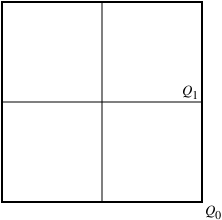
\includegraphics{HB_cube}} \hspace{0.5in} \resizebox{!}{1.25in}{\includegraphics{HB_cube_2}} \hspace{0.5in}  \resizebox{!}{1.5in}{\includegraphics{HB_cube_3}}
\end{center}
\caption{Left : $Q_1$. Middle: $Q_2$. Right: Labeling the corners.}
\label{F:Cubes}
\end{figure}
Let $Q'_0$ be one of these sub-cubes. The collection $\{O_{\alpha} \cap Q'_0\}_{\alpha \in I}$ is an open cover of $Q'_0$ in the subspace topology. If each of these open covers has a finite sub-cover, then we can take the union of all of the $O_{\alpha}$s over all of the finite sub-covers to obtain a finite sub-cover of $\{O_{\alpha}\}_{\alpha \in I}$ for $Q_0$. Since our cover $\{O_{\alpha}\}_{\alpha \in I}$ for $Q_0$ has no finite sub-cover, we conclude that there is one sub-cube, $Q_1$, for which the open cover $\{O_{\alpha} \cap Q_1\}_{\alpha \in I}$ has no finite sub-cover. Now we repeat the process and partition $Q_1$ into $2^n$ uniform sub-cubes of side length $\frac{M}{2}= \frac{2M}{2^2}$. The same argument we just made tells us that there is a sub-cube $Q_2$ of $Q_1$ for which the open cover  $\{O_{\alpha} \cap Q_2\}_{\alpha \in I}$ has no finite sub-cover (an illustration for the $n=2$ case is shown at middle in Figure \ref{F:Cubes}). We proceed inductively to obtain an infinite nested sequence 
\[Q_0 \supset Q_1 \supset Q_2 \supset Q_3 \supset \cdots \supset Q_k \supset \cdots \]
of cubes such that for each $k \in \Z$, the lengths of the sides of cube $Q_k$ are $\frac{M}{2^{k-1}} = \frac{2M}{2^{k}}$ and the open cover $\{O_{\alpha} \cap Q_k\}_{\alpha \in I}$ of $Q_k$ has no finite sub-cover. Now we show that $\bigcap_{k=1}^{\infty} Q_k \neq \emptyset$.

For $i \in \Z^+$, let $Q_i = [a_{i,1}, b_{i,1}] \times [a_{i,2}, b_{i,2}] \times \cdots [a_{i,n}, b_{i,n}]$. That is, think of the point $(a_{i,1}, a_{i,2}, \ldots, a_{i,n})$ as a lower corner of the cube and the point $(b_{i,1}, b_{i,2}, \ldots, b_{i,n})$ as an upper corner of the $n$-cube $Q_i$ (a labeling for $n=2$ and $i$ from 1 to 3 is shown at right in Figure \ref{F:Cubes}).  Let $q = (\sup\{a_{i,1}\}, \sup\{a_{i,2}\}, \ldots, \sup\{a_{i,n}\})$. We will show that $q \in \bigcap_{k=1}^{\infty} Q_k$. Fix $r \in \Z^+$. We need to demonstrate that 
\[q \in Q_r = \{(x_1, x_2, \ldots, x_n) \mid a_{r,s} \leq x_s \leq b_{r,s} \text{ for each } 1 \leq s \leq n\}.\]
For each $s$ between 1 and $n$ we have 
\begin{equation} \label{eq:cube_a}
a_{r,s} \leq \sup\{a_{i,s}\}
\end{equation}
because $\sup\{a_{i,s}\}$ is an upper bound for all of the $a_{i,s}$.  The fact that our cubes are nested means that
\begin{align}
a_{1,s} &\leq a_{2,s} \leq \cdots, \notag \\
b_{1,s} &\geq b_{2,s} \geq \cdots, \notag \\
a_{i,s} &\leq b_{i,s} \label{eq:cube_b}
\end{align}
for every $i$ and $s$. Since $\sup\{a_{i,s}\}$ is the least upper bound of all of the $a_{i,s}$, property (\ref{eq:cube_b}) shows that $\sup\{a_{i,s}\} \leq b_{i,s}$ for every $i$. Thus, $\sup\{a_{i,s}\} \leq b_{r,s}$ and so $a_{r,s} \leq \sup\{a_{i,s}\} \leq b_{r,s}$. This shows that $q \in Q_k$ for every $k$. Consequently, $q \in \bigcap_{k=1}^{\infty} Q_k$ and $\bigcap_{k=1}^{\infty} Q_k$ is not empty. (The fact that the  side lengths of our cubes are converging to 0 implies that $\bigcap_{k=1}^{\infty} Q_k = \{q\}$, but we only need to know that $\bigcap_{k=1}^{\infty} Q_k$ is not empty for our proof.)

Since $\{O_{\alpha}\}_{\alpha \in I}$ is a cover for $Q_0$, there must exist an $\alpha_q \in I$ such that $q \in O_{\alpha_q}$. The set $O_{\alpha_q}$ is open, so there exists $\epsilon_q > 0$ such that $B(q, \epsilon_q) \subseteq O_{\alpha_q}$. The maximum distance between points in $Q_k$ is the distance between the corner points $(a_{k,1}, a_{k,2}, \ldots, a_{k,n})$ and $(b_{k,1}, b_{k,2}, \ldots, b_{k,n})$, where each length $b_{k,s} - a_{k,s}$ is $\frac{M}{2^{k-1}}$. The distance formula tells us that this maximum distance between points in $Q_k$ is 
\[D_k = \sqrt{ \sum_{s=1}^n \left(\frac{M}{2^{k-1}}\right)^2} =  \sqrt{ n \left(\frac{M}{2^{k-1}}\right)^2} = \frac{M}{2^{k-1}} \sqrt{n}.\]
Now choose $K \in \Z^+$ such that $D_K < \epsilon_q$.  Then if $x \in Q_K$ we have $d_E(q,x)< D_K$ and $x \in B(q, \epsilon_q)$. So $Q_K \subseteq B(q, \epsilon_q)$. But $B(q, \epsilon_q) \subseteq O_{\alpha_q}$. So the collection $\{O_{\alpha_q} \cap Q_K\}$ is a sub-cover of $\{O_{\alpha} \cap Q_K\}_{\alpha \in I}$ for $Q_K$. But this contradicts the fact this open cover has no finite sub-cover. The assumption that led us to this contradiction was that $Q_0$ was not compact, so we conclude that the standard $n$-dimensional cube of size $M$ is a compact subset of $\R^n$ for any $M > 0$.  
\end{proof} 


One consequence of Theorem \ref{thm:Compact_cubes} is that any closed interval $[a,b]$ in $\R$ is a compact set. But we can say even more -- that the compact subsets of $\R^n$ are the closed and bounded subsets. This will require one more intermediate result about closed subsets of compact topological spaces. 


\begin{activity} Let $X$ be a compact topological space and $C$ a closed subset of $X$. In this activity we will prove that $C$ is compact. 
\ba
\item What does it take to prove that $C$ is compact? 

\item Use an open cover for $C$ and the fact that $C$ is closed to make an open cover for $X$.

\item Use the fact that $X$ is compact to complete the proof of the following theorem.

\begin{theorem} \label{thm:closed_compact} Let $X$ be a compact topological space. Then any closed subset of $X$ is compact. 
\end{theorem}

\ea

\end{activity}

\begin{comment}

\ActivitySolution

\ba
\item We need to show that every open cover of $C$ has a finite subcover. 

\item Let $\{O_{\alpha}\}$ be an open cover of $C$ for $\alpha$ in some indexing set $I$. Since $C$ is closed, the set $X \setminus C$ is an open set. Then $\{O_{\alpha}\} \cup (X \setminus C)$ is an open cover of $X$.

\item Since $X$ is compact, this open cover has a finite sub-cover. In other words, there are sets $O_{\alpha_1}$, $O_{\alpha_2}$, $\ldots$, $O_{\alpha_n}$ for some positive integer $n$ such that $\alpha_i \in I$ for each $i$ and 
\[X \subseteq O_{\alpha_1} \cup O_{\alpha_2} \cup \cdots \cup O_{\alpha_n} \cup (X \setminus C).\]
But then we must have
\[C \subseteq O_{\alpha_1} \cup O_{\alpha_2} \cup \cdots \cup O_{\alpha_n}\]
and we have found a finite sub-cover of the open cover $\{O_{\alpha}\}$. We conclude that $C$ is compact.

\ea

\end{comment}

Now we can prove a major result, that the compact subsets of $(\R^n, d_E)$ are the closed and bounded subsets. This result is important enough that it is given a name. 

\begin{theorem}[The Heine-Borel Theorem] A subset $A$ of $(\R^n, d_E)$ is compact if and only if $A$ is closed and bounded. 
\end{theorem}

\begin{proof} Let $A$ be a subset of $(\R^n, d_E)$. Assume that $A$ is closed and bounded. Since $A$ is bounded, there is a positive number $M$ such that $A \subseteq Q^n_M$. Theorem \ref{thm:Compact_cubes} shows that $ Q^n_M$ is compact, and then Theorem \ref{thm:closed_compact} shows that $A$ is compact. 

For the converse, assume that $A$ is a compact subset of $\R^n$. We must show that $A$ is closed and bounded. Now $(\R^n, d_E)$ is a metric space, and so Hausdorff. Theorem \ref{thm:metric_compact_closed} then shows that $A$ is closed. To conclude our proof, we need to demonstrate that $A$ is bounded. For each $k > 0$, let 
\[O_k = \{ (x_1,x_2, \ldots, x_n) \mid -k < x_i < k \text{ for every } 1 \leq i \leq n\}.\]
That is, $O_k$ is the open $k$-cube in $\R^n$. Next let 
\[U_k = O_k \cap A\]
for each $k$. Since $\bigcup_{k > 0} O_k = \R^n$, it follows that $\{U_k\}_{k > 0}$ is an open cover of $A$. The fact that $A$ is compact means that there is a finite collection $U_{k_1}$, $U_{k_2}$, $\ldots$, $U_{k_m}$ of sets in $\{U_k\}_{k > 0}$ that cover $A$. Let $K = \max\{k_i \mid 1 \leq i \leq m\}$. Then $U_{k_i} \subseteq U_K$ for each $i$, and so $A \subseteq U_K \subset Q^m_K$. Thus, $A$ is bounded. This completes the proof that if $A$ is compact in $\R^n$, then $A$ is closed and bounded. 
\end{proof}

You might wonder whether the Heine-Borel Theorem is true in any metric space.

\begin{activity} A subset $A$ of a metric space $(X, d)$ is bounded if there exists a real number $M$ such that $d(a_1,a_2) \leq M$ for all $a_1, a_2 \in A$. (This is equivalent to our definition of a bounded subset of $\R^n$ given earlier, but works in any metric space.) Explain why $\Z$ as a subset of $(\R,d)$, where $d$ is the discrete metric, is closed and bounded but not compact.  

\end{activity}

\begin{comment}

\ActivitySolution Let $M = 1$. For any $a_1, a_2 \in \Z$, we have that $d(a_1,a_2) \leq 1$. So $\Z$ is bounded. Every subset of a metric space with the discrete metric is closed, so $\Z$ is closed.  But $\Z$ is not compact since open cover with no finite sub-cover is $\{\{n\}\}_{n \in \Z}$. 

\end{comment}
 

\csection{An Application of Compactness}\label{sec_compact_app}

As mentioned at the beginning of this section, compactness is the quality we need to ensure that continuous functions from topological spaces to $\R$ attain their maximum and minimum values.


\begin{activity} In this activity we prove the following theorem. 

\begin{theorem} \label{thm:max_min} A continuous function from a compact topological space to the real numbers assumes a maximum and minimum value. 
\end{theorem}

\ba
\item Let $X$ be a compact topological space and $f: X \to \R$ a continuous function. What does the continuity of $f$ tell us about $f(X)$ in $\R$? 

\item Why can we conclude that the set $f(X)$ has a least upper bound $M$? Why must $M$ be an element of $f(X)$?

\item Complete the proof of Theorem \ref{thm:max_min}.

\ea

\end{activity}

\begin{comment}

\ActivitySolution

\ba
\item Since $f$ is continuous, we know that $f(X)$ is compact in $\R$ by Activity 16.2. 

\item By the Heine-Borel Theorem, it follows that $f(X)$ is closed and bounded. Since $f(X)$ is bounded, there is a least upper bound $M$ for $f(X)$. Now $M$ is a limit point of $f(X)$ and $f(X)$ is closed, so $M \in f(X)$.

\item Similarly, $f(X)$ contains its greatest lower bound $m$. Thus, $f$ assumes a maximum value $M$ and a minimum value $m$ in $\R$.

\ea


\end{comment}


\csection{Summary}\label{sec_compact_top_summ}
Important ideas that we discussed in this section include the following.
\begin{itemize}
\item A cover of a subset $A$ of a topological space $X$ is any collection of subsets of $X$ whose union contains $A$. An open cover is a cover consisting of open sets. 
\item A subcover of a cover of a set $A$ is a subset of the cover such that the union of the sets in the subcover also contains $A$.
\item A subset $A$ of a topological space is compact if every open cover of $A$ has a finite subcover. 
\item A continuous function from a compact topological space to the real numbers must attain a maximum and minimum value. 
\item The Heine-Borel Theorem states that the compact subsets of $\R^n$ are exactly the subsets that are closed and bounded. 
\end{itemize}


\csection{Exercises}\label{sec_compact_top_exer}

\be

\item 
	\ba
	\item Determine the compact subsets of a topological space $X$ with the indiscrete topology.
	
	\item Determine the compact subsets of a topological space $X$ with the indiscrete topology.
	
	\ea

\begin{comment}
	
\ExerciseSolution

\ba

\item Let $X$ be a topological space with the discrete topology, and let $A$ be a nonempty subset of $X$. If $\{O_{\alpha}\}_{\alpha \in I}$ is an open cover of $A$, then at least one of the open sets must be $X$. So $\{X\}$ is a finite subcover of $A$. This shows that every subset of $X$ is compact. 

\item Let $X$ be a topological space with the discrete topology. We know that finite sets are compact, so suppose that $A$ is an infinite subset of $X$. Every subset of $X$ is open, so the collection $\{\{a\}\}_{a \in A}$ is an open cover of $A$. But if we eliminate any set from this open cover, the resulting collection won't cover $A$. So we have found an open cover of $A$ with no finite subcover. We conclude that the only compact subsets of $X$ are the finite subsets. 

\ea

\end{comment}


\item Recall from Definition \ref{def:weaker_topologies} on page \pageref{def:weaker_topologies} that if $\tau_1$ and $\tau_2$ are two topologies on a set $X$ such that $\tau_1 \subseteq \tau_2$, then $\tau_1$ is said to be a \emph{coarser} (or \emph{weaker}) topology than $\tau_2$, or $\tau_2$ is a \emph{finer} (or \emph{stronger}) topology than $\tau_1$. In this exercise we explore the question of whether compactness is a property that is passed from weaker to stronger topologies or from stronger to weaker. 

Let $\tau_1$ and $\tau_2$ be two topologies on a set $X$. If $\tau_1 \subseteq \tau_2$, what does compactness under $\tau_1$ or $\tau_2$ imply, if anything, about compactness under the other topology? Justify your answers.


\begin{comment}

\ExerciseSolution Let $A$ be a subset of $X$ and suppose $A$ is compact in $(X, \tau_2)$. If $\{O_{\alpha}\}_{\alpha \in I}$ is an open cover of $A$ in $(X, \tau_1)$, then $\{O_{\alpha}\}_{\alpha \in I}$ is also an open cover of $A$ in $(X, \tau_2)$. Since $A$ is compact in $(X, \tau_2)$, there is a finite subcover $\{O_{\alpha_k}\}_{1 \leq k \leq n}$ of  $\{O_{\alpha}\}_{\alpha \in I}$. Thus, $A$ is also compact in $(X, \tau_1)$. 

However, if $A$ is compact in $(X, \tau_1)$, it does not follow that $A$ is compact in $(X,\tau_2)$. For example, consider $X = \R$ with $\tau_1$ the Euclidean metric topology and $\tau_2$ the discrete topology. We know that $[0,1]$ is compact in $(X, \tau_1)$, but the open cover $\{n\}_{n \in [0,1]}$ for $[0,1]$ in $(X, \tau_2)$ has no finite subcover. 


\end{comment}

\item \label{ex:intersection_not_compact} Let $\E$ be the set of even integers, and let $\tau = \{\Z\} \cup \{O \subseteq \E\}$. That is, $\tau$ is the collection of all subsets of $\E$ along with $\Z$. 
\ba
\item Prove that $\tau$ is a topology on $\Z$.

\item Find all compact subsets of $(\Z, \tau)$. Verify your answer.

\item Prove or disprove: If $A$ and $B$ are compact subsets of a topological space $X$, then $A \cap B$ is also a compact subset of $X$.

\ea

\begin{comment}

\ExerciseSolution

\ba

\item By definition, $\Z \in \tau$. Since $\emptyset \subset \E$ it is also the case that $\emptyset \in \tau$. Now let $O_{\alpha}$ be elements of $\tau$ for $\alpha$ in some indexing set $I$. If $O_{\beta} = \Z$ for some $\beta \in I$, then $\bigcup_{\alpha \in I} O_{\alpha} = \Z \in \tau$. So assume that $O_{\alpha} \neq \Z$ for all $\alpha \in I$. Suppose $x \in \bigcup_{\alpha \in I} O_{\alpha}$. Then $x \in O_{\beta}$ for some $\beta \in I$. This means that $x \in O_{\beta} \subseteq \E$ and $x$ is even. Thus,  $\bigcup_{\alpha \in I} O_{\alpha} \subseteq \E$ and so $\bigcup_{\alpha \in I} O_{\alpha}$ is in $\tau$. Now suppose that $I$ is finite. If $O_{\alpha} = \Z$ for every $\alpha \in I$, then $\bigcap_{\alpha \in I} O_{\alpha} = \Z \in \tau$. Assume $O_{\alpha} \neq \Z$, for some $\alpha \in I$. Suppose that $x \in \bigcap_{\alpha \in I} O_{\alpha}$. Then $x \in O_{\alpha}$ for every $\alpha \in I$.   But this again means that $x$ is even and $\bigcap_{\alpha \in I} O_{\alpha} \subseteq \E$. We conclude that $\tau$ is a topology on $\Z$. 

\item We will show that a set $C$ in $(\Z, \tau)$ is compact if and only if $C$ is a finite set of even integers or $C$ contains at least one odd integer. 

First assume that $C$ is a compact subset of $(\Z, \tau)$. We proceed by contradiction and assume that $|C|$ is infinite and that $C \subseteq \E$. For each $m \in C$, let $O_m = \{m\}$. Since the elements of $C$ are even, every $O_m$ is in $\tau$. Thus, $\{O_m\}_{m \in C}$ is an open cover of $C$. If $m\in C$ and we removing $O_m$ from this cover, then the resulting union does not contain $m$. So the open cover $\{O_m\}_{m \in C}$ has no finite subcover and $C$ is not compact.

We know that every finite set is compact, so to prove the reverse implication assume that $C$ is a subset of $\Z$ that contains an odd integer $n$. Let $\{O_{\alpha}\}_{\alpha \in I}$ be an open cover of $C$ for $\alpha$ in some indexing set $I$. Thus, $n \in \bigcup_{\alpha \in I} O_{\alpha}$. But the only open set that contains $n$ is $\Z$ itself, so there exists $\beta \in I$ such that $O_{\beta} = \Z$. But then $\{\Z\}$ is a finite subcover of $\{O_{\alpha}\}_{\alpha \in I}$. We conclude that $C$ is compact. 

\item It is not true that if $A$ and $B$ are compact subsets of a topological space $X$, then $A \cap B$ is compact. Consider $A = \{1\} \cup \E$ and $B = \{3\} \cup \E$ in $(\Z, \tau)$. Both $A$ and $B$ are compact by part (b) of this problem, but $A \cap B = \E$ is not compact. 


\ea


\end{comment}


\item Let $(X,\tau)$ be a topological space

\ba

\item Prove that the union of any finite number of compact subsets of $X$ is a compact subset of $X$.

\item In Exercise (\ref{ex:intersection_not_compact}) we should have seen that the intersection of compact sets is not necessarily compact. If $X$ is Hausdorff, prove that the intersection of any finite number of compact subsets of $X$ is a compact subset of $X$.

\ea

\begin{comment}

\ExerciseSolution

\ba

\item Let $n$ be a positive integer and let $C_1$, $C_2$, $\ldots$, $C_n$ be compact subsets of $X$. Suppose $\{O_{\alpha}\}_{\alpha \in I}$ is an open cover of $\bigcup_{1 \leq k \leq n} C_k$. Let $k$ be between $1$ and $n$. Then $\{O_{\alpha}\}_{\alpha \in I}$ is an open cover of $C_k$. Since $C_k$ is compact, there is an open subcover $\{O_{\gamma}\}_{\gamma \in J_k}$ of $C_k$ for some finite set $J_k$. Thus, $\{O_{\delta}\}_{\delta \in \cup_{1 \leq i \leq n} J_k}$ is a finite subcover of $\bigcup_{1 \leq k \leq n} C_k$. 

\item Assume that $X$ is Hausdorff, let $n$ be a positive integer, and let $C_1$, $C_2$, $\ldots$, $C_n$ be compact subsets of $X$. Suppose $\{O_{\alpha}\}_{\alpha \in I}$ is an open cover of $\bigcap_{1 \leq k \leq n} C_k$. Let $m$ be between $1$ and $n$. Since $C_m$ is a compact subset of a Hausdorff space, we know that $C_m$ is closed. Thus, $X \setminus C_m$ is open. Recall that $X \setminus \bigcap_{1 \leq k \leq n} C_k = \bigcup_{1 \leq k \leq n} (X \setminus C_k)$, so $O = X \setminus \bigcap_{1 \leq k \leq n} C_k$ is open. Since $\bigcap_{1 \leq K \leq N} C_k \subseteq \bigcup_{\alpha \in I} O_{\alpha}$, it follows that $X = O \cup \left(\bigcup_{\alpha \in I} O_{\alpha} \right)$ and so $\{O\} \cup \{O_{\alpha}\}_{\alpha \in I} $ is an open cover for $C_m$. Since $C_m$ is compact, this open cover has a finite subcover. Let $\{O_{i}\}_{i \in J_m}$ be the finite collection of the $O_{\alpha}$ in this subcover. The fact that $O \bigcap \bigcap_{1 \leq k \leq n} C_k = \emptyset$ implies that $\bigcap_{1 \leq k \leq n} C_k \subseteq \bigcup_{i \in J_m} O_{i}$. Thus, $\{O_{i}\}_{i \in J_m}$ is a finite subcover of $\{O_{\alpha}\}_{\alpha \in I}$ and $\bigcap_{1 \leq k \leq n} C_k$ is a compact set. 


\ea

\end{comment}

\item Consider $\Z$ with the digital line topology (see Exercise (\ref{ex:digital_line_topology}) on page \pageref{ex:digital_line_topology}). Determine the compact subsets of $\Z$. 

\begin{comment}

\ExerciseSolution We will show that the only compact subsets of $\Z$ are the finite subsets. Since we know that finite sets are compact, we only need to verify that no infinite subset of $\Z$ is compact. Let $A$ be an infinite subset of $\Z$. Recall that a basis for the digital line topology on $\Z$ is the collection $\{B(n)\}$, where $B(n) = \{n\}$ if $n$ is odd and $B(n) = \{n-1,n,n+1\}$ if $n$ is even. So $\{B(n)\}_{n \in A}$ is an open cover of $A$. Since each $B(n)$ is finite, any finite subcollection of sets in $\{B(n)\}_{n \in A}$ will have a finite union and can't form a cover of $A$. We conclude that $A$ is not compact. 

\end{comment}

\item For each $n \in \Z^+$, let $(-n,n)$ be the set of integers in the interval $(-n,n)$ (see Exercise (\ref{ex:coarse_topology_example}) on \pageref{ex:coarse_topology_example}.)  
	\ba
	\item Show that $\B = \{(-n,n)\}_{n \in \Z^+}$ is a basis for a topology $\tau$ on $\Z$
	
	\item Is the subset $(-2,2)$ compact in this topology?
	
	\item Determine all of the compact subsets of $\Z$.
	
	\ea

\begin{comment}

\ExerciseSolution

	\ba
	\item First, $0 \in (-1,1)$. If $n \in \Z$ is not zero, then $n \in (-|n|+1, |n|+1)$. 
	
	Now suppose that $B_1$ and $B_2$ are basis sets and $n \in B_1 \cap B_2$. As basis sets, we know that $B_1 = (-k,k)$ and $B_2 = (-m,m)$ for some $k, mm \in \Z^+$. Without loss of generality, assume that $k \leq m$. Then $B_1 \subseteq B_2$ and $n \in B_1 = B_1 \cap B_2$. 
So $\B$ is a basis for a topology on $\Z$.	

	\item Let $\{O_{\alpha}\}_{\alpha \in I}$ for $\alpha$ in some indexing set $I$ be an open cover of $(2,2)$. Each $O_{\alpha}$ is a union of basis sets, so the open cover $\{O_{\alpha}\}_{\alpha \in I}$ also has the form $\{(-n,n)\}_{n \in J}$ for some subset $J$ of $\Z^+$. Since the sets $(-n,n)$ for $n \in J$ cover $(-2,2)$, there is an integer $m \in J$ such that $m > 2$. Thus, $\{(-m,m)\}$ is a finite subcover of $(-2,2)$ in $\{(-n,n)\}_{n \in J}$. We conclude that $(-2,2)$ is a compact subset of $\Z$. 
		
	\item We will show that the subsets of $\Z$ that are compact are finite subsets. It suffices to show that no infinite subset of $\Z$ is compact. Let $A$ be an infinite subset of $\Z$ and let $\{O_{\alpha}\}_{\alpha \in I}$ for $\alpha$ in some indexing set $I$ be an open cover of $A$. Each $O_{\alpha}$ is a union of basis sets, so the open cover $\{O_{\alpha}\}_{\alpha \in I}$ also has the form $\{(-n,n)\}_{n \in J}$ for some subset $J$ of $\Z^+$. Suppose there is a finite subcover $\{(-n,n)\}_{n \in K}$ of $A$ in $\{(-n,n)\}_{n \in J}$. Let $m = \max\{n \mid n \in K\}$. Then $(-n,n) \subseteq (-m,m)$ for every $n \in K$. But $(-m,m)$ is a finite set of integers, and so can't cover the infinite set $A$. We conclude that $A$ is not compact. 
	
	\ea

\end{comment}

\item Let $X$ and $Y$ be topological spaces, and let $f: X \to Y$ be a function.

\ba

\item Suppose that $f$ is a continuous function, and that $X$ is compact and $Y$ is Hausdorff. Prove that if $C$ is a closed subset of $X$, then $f(C)$ is a closed subset of $Y$. (Thus, $f$ is a \emph{closed} function.) (Hint: Use Activity 17.3, Activity 17.4, and Theorem 17.6.)

\item Suppose that $f$ is a continuous bijection. Prove that if $X$ is compact and $Y$ is Hausdorff, then $f$ is a homeomorphism.

\item Give an example where $f$ is a continuous bijection and $X$ is compact, but $f$ is not a homeomorphism.

\item Give an example where $f$ is a continuous bijection and $Y$ is Hausdorff, but $f$ is not a homeomorphism.

\ea

\begin{comment}

\ExerciseSolution

\ba

\item Let $C$ be a closed subset of $X$. Activity 17.4 shows that closed subsets of a compact space are compact, so we know that $C$ is compact. Activity 17.2 shows that $f(C)$ is compact. Since $Y$ is Hausdorff, Theorem 17.6 allows us to conclude that that $f(C)$ is closed. So $f$ sends closed sets to closed sets. 

\item To show that $f^{-1}$ is continuous, we use the result of Exercise \ref{ex:continuity_closed_topology} on page \pageref{ex:continuity_closed_topology} and show that $(f^{-1})^{-1}(C)$ is closed in $Y$ whenever $C$ is closed in $X$. Let $C$ be a closed set in $X$. Part (a) shows that $f(C)$ is also closed. But $f$ is a bijection, so $C = (f^{-1})^{-1}(C)$. 

\item Let $X = \{a,b,c,d\} = Y$, let $\tau_X$ be the discrete topology on $X$ and $\tau_Y = \{\emptyset, \{a\}, \{b,c\}, \{a,b,c\}, Y\}$ the topology on $Y$. As a finite space, we know that $X$ is compact. Since $\{b\}$ is not a closed set, we know that $Y$ is not a Hausdorff space. Define $f: X \to Y$ by $f(x) = x$ for all $x \in X$. Then $f$ is the identity function, so is a bijection. The fact that every subset of $X$ is open means that $f$ is continuous. But $\{b\}$ is an open set in $X$ while $f(\{b\} = \{b\}$ is not an open set in $Y$. Thus, $f$ is not an open function and not a homeomorphism.

\item Let $X = \R = Y$, let $\tau_X$ be the discrete topology on $X$ and $\tau_Y$ the Euclidean topology on $Y$. As an infinite space with the discrete metric, we know that $X$ is not compact. Since $Y$ is a metric space we know that $Y$ is Hausdorff. Define $f: X \to Y$ by $f(x) = x$ for all $x \in X$. Then $f$ is the identity function, so is a bijection. The fact that every subset of $X$ is open means that $f$ is continuous. But the set $\{0\}$ is an open set in $X$ while $f(\{0\} = \{0\}$ is not an open set in $Y$. Thus, $f$ is not an open function and not a homeomorphism.

\ea

\end{comment}


\item The Either-Or topology on the interval $X = [-1,1]$ has as its open sets all subsets of $X$ that contain $(-1,1)$ and any subset of $X$ that doesn't contain $0$. 
\ba

\item Describe the non-trivial closed subsets of $X$.

\item Is $X$ a Hausdorff topological space? Explain.

\item Is $X$ compact? Prove your answer.

\item Are there any subsets of $\Z$ that are not compact? Justify your answer. 

\ea

\begin{comment}

\ExerciseSolution

\ba

\item If $A$ is a subset of $X$ that contains $0$, then $X \setminus A$ doesn't contain $0$ and is therefore open. The complement of $\{-1,1\}$ is $(-1,1)$, which is open. The complement of $\{-1\}$ is $(-1,1] = (-1,1) \cup \{1\}$, which is open. The complement of $\{1\}$ is $[-1,1) = \{-1\} \cup (-1,1)$, which is open. To show that these are the only non-trivial closed sets, suppose that $A$ is a closed subset of $X$ that doesn't contain $0$. Then $X \setminus A$ contains $0$. The only open set that contains $0$ is $(-1,1)$, and so $X \setminus A$ must be equal to $(-1,1) \cup O$ for some open set $O$. This implies that $A$ is a subset of $\{-1,1\}$. 

\item Since not all single point sets are closed in $X$, we conclude that $X$ is not a Hausdorff space. 

\item Suppose $\{O_{\alpha}\}_{\alpha \in I}$ is an open cover of $\Z$. Let $O_1$ be one of the $O_{\alpha}$ that contains $0$. It follows that $(-1,1) \subseteq O_1$.  Now let $O_2$ be one of the $O_{\alpha}$ that contains $-1$ and $O_3$ one of the $O_{\alpha}$ that contains $1$. Then $\{O_1, O_2, O_3\}$ is a finite subcover of $\{O_{\alpha}\}_{\alpha \in I}$. We conclude that $\Z$ is compact. 

\item Recall that closed subsets of compact spaces are compact. So we look for a subset of $X$ that is not closed. Let $A = X \setminus \{0\}$. If $a \in A$, we know that $\{a\}$ is an open set. Then $\{\{a\}\}_{a \in A}$ is an open cover of $A$ with no finite subcover. So $A$ is not compact.  

\ea

\end{comment}


\item \label{ex:Compact_normal} Let $X$ be a topological space.

\ba

\item Prove that if $X$ is Hausdorff and $C$ is a compact subset of $X$, then for each $x \in X \setminus C$ there exist disjoint open sets $U$ and $V$ such that $x \in U$ and $C \subseteq V$. 

\item Prove that if $X$ is a compact Hausdorff space, then $X$ is normal.

\ea

\begin{comment}

\ExerciseSolution 

\ba

\item Assume that $X$ is Hausdorff and let $C$ be a compact subset of $X$. Let $x \in X \setminus C$. As a compact subset of a Hausdorff space, $C$ is closed. So $X \setminus C$ is open. Let $y \in C$. Then there exist disjoint open sets $U_y$ and $V_y$ such that $x \in U_y$ and $y \in V_y$. So $\{V_y\}_{y \in C}$ is an open cover of $C$. Since $C$ is compact, there exist $y_1$, $y_2$, $\ldots$, $y_n$ in $Y$ such that $\{V_{y_i}\}_{1 \leq i \leq n}$ is a finite subcover of $\{V_y\}_{y \in C}$. Let $V = \bigcup_{1 \leq i \leq n} V_{y_i}$ and let $U = \bigcap_{1 \leq i \leq n} U_{y_i}$. Since $U \cap V_{y_i} \subseteq U_{y_i} \cap V_{y_i} = \emptyset$ for each $i$, it follows that $U \cap V = \emptyset$. Also, $x \in U_{y_i}$ for each $i$ implies that $x \in U$. So $U$ and $V$ are the desired sets.  

\item Let $X$ be a compact Hausdorff space, and let $C$ and $D$ be closed subsets of $X$. Every closed subset of a compact space is compact, so both $C$ and $D$ are compact. For each $x \in C$, part (a) provides disjoint open sets $U_x$ and $V_x$ such that $x \in U_x$ and $D \subseteq V_x$. Thus, $C \subseteq \bigcup_{x \in C} U_x$. Since $C$ is compact, there exist $x_1$, $x_2$, $\ldots$, $x_n$ in $C$ such that $C \subseteq \bigcup_{1 \leq i \leq n} U_{x_i}$. Let $U = \bigcup_{1 \leq i \leq n} U_{x_i}$ and $V = \bigcap_{1 \leq i \leq n} V_{x_i}$. Since $D \subseteq V_{x_i}$ for each $i$, $D \subseteq V$. The fact that $U \cap V_{x_i} \subseteq U_{x_i} \cap V_{x_i} = \emptyset$ for each $i$ implies that $U \cap V = \emptyset$. Thus, the open sets $U$ and $V$ separate the closed sets $C$ and $D$. We conclude that $X$ is normal. 

\ea

\end{comment}


\item Let $X$ be a nonempty set and let $p$ be a fixed element in $X$. Let $\tau_p$ be the particular point topology and $\tau_{\overline{p}}$ the excluded point topology on $X$. That is
\begin{itemize}
\item $\tau_{p}$ is the collection of subsets of $X$ consisting of $\emptyset$, $X$, and all of the subsets of $X$ that contain $p$.  
\item $\tau_{\overline{p}}$ is the collection of subsets of $X$ consisting of $\emptyset$, $X$, and all of the subsets of $X$ that do not contain $p$.
\end{itemize}
That the particular point and excluded point topologies are topologies is the subject of Exercises (\ref{ex:particular_point_topology}) and (\ref{ex:excluded_point_topology}) on page \pageref{ex:particular_point_topology}. 

Determine, with proof, the compact subsets of $X$ when 
\ba
\item $X$ has the particular point topology $\tau_p$

\item $X$ has the excluded point topology $\tau_{\overline{p}}$. 

\ea

\begin{comment}

\ExerciseSolution We know that any finite set is compact, so assume from this point on that $X$ is an infinite set.

\ba
	\item If $C$ is a finite subset of $X$, then $C$ is compact. We claim that no infinite subset $C$ of $X$ is compact. Assume that $C$ is an infinite subset of $X$. For each $c$ in $C$, let $O_c = \{p,c\}$.  Since $p \in O_c$ for each $c$, we conclude that $O_c$ is an open set. Thus, $\mathcal{O} = \{O_c \mid c \in C\}$ is an open cover for $C$. If $\{O_{\alpha}\}$ is a finite subset of $\mathcal{O}$, then $\bigcup O_{\alpha}$ is finite set and cannot cover the infinite set $C$. Thus, the open cover $\mathcal{O}$ of $C$ has no finite subcover and $C$ is not a compact subset of $(X \tau_p)$. Therefore, the only compact subsets of $(X, \tau_p)$ are the finite subsets.
	
	\item If $C$ is a finite subset of $X$, then $C$ is compact. Assume that $C$ is an infinite subset of $X$. We will show that $C$ is compact if and only if $p \in C$. 
	
	First assume that $p \in C$. Let $\{O_{\alpha}\}_{\alpha \in I}$ be an open cover of $C$. Then $p \in O_{\alpha}$ for some $\alpha \in I$. The only open set that contains $p$ is $X$, so $O_{\alpha} = X$. Then $\{X\}$ is an open subcover of the open cover $\{O_{\alpha}\}_{\alpha \in I}$. Thus, $C$ is compact in $(X, \tau_{\overline{p}})$. 
	
	Now assume that $p \notin C$. Let $O_c = \{c\}$ for every $c \in C$. Since $p \notin C$ we know that $O_c$ is in $\tau_{\overline{p}}$. Let $\mathcal{O} = \{O_c\}_{c \in C}$. Then $\mathcal{O}$ is an open cover of $C$ that has no finite subcover. Thus $C$ is not compact. 
	
	We conclude that the compact subsets of $(X, \tau_{\overline{p}})$ are the finite sets and the infinite sets that contain $p$.  
	
	\ea



\end{comment}

\item In this exercise we encounter a non-Hausdorff topological space in which single points sets are closed, and in which compact subsets need not be closed. Consider the set $\Z$ with the finite complement topology $\tau_{FC}$.  

\ba

\item Show that every single point set is closed.

\item Explain why $(\Z, \tau_{FC})$ is not a Hausdorff space. 

\item Let $U$ be an open set in $(\Z, \tau_{FC})$ that contains $0$ and $V$ an open set in $(\Z, \tau_{FC})$ that contains $1$. Explain why it cannot be the case that $U$ and $V$ are disjoint -- that is, $U \cap V$ must be non-empty.

\item Show that the subset $\E$ of even integers is a compact subset of $(\Z, \tau_{FC})$ that is not closed. Verify your result.

\ea


\begin{comment}

\ExerciseSolution 

\ba

\item Let $n \in \Z$. Since the complement of $\Z \setminus \{n\}$ is just the finite set $\{n\}$, we see that $\Z \setminus \{n\}$ is an open set. We conclude that $\{n\}$ is a closed set.

\item Let $x$ and $y$ be distinct points in $\Z$. Let $O_x$ be an open set containing $x$ and  $O_y$ an open set containing $y$. Then $\Z \setminus O_x$ and $\Z \setminus O_y$ are both finite. Let $\Z \setminus O_x = \{r_1, r_2, \ldots, r_k\}$ and let $\Z \setminus O_y = \{s_1, s_2, \ldots, s_m}$. So if $z \notin \{r_1, r_2, \ldots, r_k, s_1, s_2, \ldots, s_m\}$, then $z \in O_x \cap O_y$. Thus, it is impossible to find two disjoint open sets that separate $x$ and $y$, and $(\Z, \tau_{FC})$ is not Hausdorff.  

\item Since $U$ and $V$ are open, we know that $U$ and $V$ each contain all but a finite number of elements in $\Z$. That is, $\Z \setminus U = \{u_1, u_2, \ldots, u_m\}$ and $\Z \setminus V = \{v_1, v_2, \ldots, v_n\}$ for some integers $u_i$ and $v_j$. So if $x \notin \{u_1,u_2, \ldots, u_m, v_1, v_2, \ldots, v_n\}$, then $x \in U \cap V$. So $U$ and $V$ can't be disjoint.

\item Let $\E$ be the set of even integers. The complement of $\E$ is the set $\Odd$ of odd integers, and $\Z \setminus \Odd = \E$ is not finite, so $\Odd$ isn't an open set. Thus, $\E$ is not a closed set.

Now we show that $\E$ is compact. Let $\{O_{\alpha}\}_{\alpha \in I}$ be a collection of open sets for $\alpha$ in some indexing set $I$ whose union contains $\E$. Choose as set in $\{O_{\alpha}\}_{\alpha \in I}$ and label it as $O_1$. The fact that $O_1$ is open means that $\E \setminus O_1 \subseteq \Z \setminus O_1$ is finite. Let $\E \setminus O_1 = \{a_2, a_3, \ldots, a_n\}$. For each $i$ from $2$ to $n$, let $O_i be in $\{O_{\alpha}\}_{\alpha \in I}$ such that $a_i \in O_i$. It follows that $\E \subseteq \bigcup_{i=1}^n O_i$ and the set $\{O_i}_{i=1}^n$ is a finite subcover of $\E$ in $\{O_{\alpha}\}_{\alpha \in I}$. We conclude that $\E$ is compact. 

\ea


\end{comment}

\item Let $(X, \tau)$ be a Hausdorff topological space.

\ba

\item Let $x \in X$ and let $A$ be a compact subset of $X$. Prove that there exist disjoint open subsets $U$ and $V$ of $X$ such that $x \in U$ and $A \subseteq V$. 

\item Let $A$ and $B$ be disjoint compact subsets of $X$. Prove that there exist disjoint open sets $U$ and $V$ such that $A \subseteq U$ and $B \subseteq V$. 

\ea

\begin{comment}

\ExerciseSolution 

\ba

\item Let $a \in A$. Since $X$ is Hausdorff, there exist disjoint open sets $O_{x_a}$ and $O_a$ such that $x \in O_{x_a}$ and $a \in O_a$. Now $\{O_a\}_{a \in A}$ is an open cover of $A$. Since $A$ is compact, there is a finite subcover $\{O_{a_i}\}_{1 \leq i \leq n}$ for $A$ of $\{O_a\}_{a \in A}$. Let $V = \bigcup_{i=1}^n O_{a_i}$. Then $V$ is an open set and $A \subseteq V$. Now let $U = \bigcap_{i=1}^n O_{x_{a_i}}$. As a finite intersection of open sets, we know that $U$ is an open set. The fact that $x \in O_{a_i}$ for each $i$ means that $x \in U$. To complete our proof, we will demonstrate that $U \cap V = \emptyset$. Suppose $z \in U \cap V$. Since $z \in V$, there is an integer $k$ such that $z \in O_{a_k}$. Because $z in U$, we know that $z \in O_{x_{a_k}}$, But $O_{x_{a_k}} \cap O_{a_k} = \emptyset$. We conclude that $U \cap V = \emptyset$.  


\item By part (a), for each $b \in B$ there exists open sets $U_b$ and $V_b$ such that $A \subseteq U_b$ and $b \in V_b$. The collection $\{V_b\}_{b \in B}$ is an open cover of $B$. Because $B$ is compact, there is a finite subcover $\{V_{b_i}\}{1 \leq i \leq n}$ for $B$. As in part (a) the sets $V = \bigcup_{i=1}^n V_{b_i}$ and $U = \bigcap_{i=1}^n U_{b_i}$ are disjoint, and $A \subseteq U$ and $B \subseteq V$.  

\ea

\end{comment}

\item \label{ex:subspace_compact} Let $(X,\tau_X)$ be a topological space and let $A$ be a subset of $X$. Let $\tau_A$ be the subspace topology on $A$. Prove that $A$ is a compact subset of $X$ if and only if $(A, \tau_A)$ is a compact topological space. 

\begin{comment}

\ExerciseSolution First, suppose that $A$ is a compact subset of $X$. To show that $(A, \tau_A)$ is a compact space, let $\{O_{\alpha}\}$, for $\alpha$ in some indexing set $I$, be an open cover of $A$ in the subspace topology. Then, for each $\alpha \in I$ there exists an open set $U_{\alpha}$ of $X$ such that $O_{\alpha} = U_{\alpha} \cap A$. Since $A \subseteq \bigcap_{\alpha \in I} O_{\alpha}$ it follows that $A \subseteq \bigcap_{\alpha \in I} U_{\alpha}$. The fact that $A$ is a compact subset of $X$ implies that there is a finite subcover $\{U_i\}_{i = 1|^n$ for $A$ of the open cover $\{U_{\alpha}\}_{\alpha \in I}$. So $A \subseteq \bigcap_{1 \leq i \leq n} U_{i}$. From this we have $A =  \bigcap_{1 \leq i \leq n} (U_{i} \cap A) = \bigcap_{1 \leq i \leq n} O_{i}$ and we have found a finite subcover for $A$ of the open cover $\{O_{\alpha}\}$. We conclude that $(A, \tau_A)$ is a compact topological space. 

For the reverse implication, assume that $A$ is a compact topological space. To prove that $A$ is a compact subset of $X$, let $\{U_{\alpha}\}$, for $\alpha$ in some indexing set $I$, be an open cover of $A$ in $(X, \tau_X)$. For each $\alpha \in I$, let $O_{\alpha} = U_{\alpha} \cap A$. Then $O_{\alpha$ \in \tau_A$ for each $\alpha in I$ and $A = \bigcup_{\alpha in I} O_{\alpha}$. But $(A, \tau_A)$ is a compact topological space, so there is a finite subcover $\{O_i\}_{1 \leq i \leq n}$ for $A$ of $\{O_{\alpha}\}_{\alpha \in I}$. That is, $A = \bigcup_{1 \leq i \leq n} O_i = \bigcup_{1 \leq i \leq n} (U_i \cap A)$. so $A \subseteq \bigcup_{1 \leq i \leq n} U_i$, and there is a finite subcover for $A$ of the open cover $\{U_{\alpha}\}$. We conclude that $A$ is a compact subset of $X$. 

\end{comment}


\item Let $X$ be a topological space. A family $\{F_{\alpha}\}_{\alpha \in I}$ of subsets of $X$ is said to have the \emph{finite intersection property} if for each finite subset $J$ of $I$, $\bigcap_{\alpha \in J} F_{\alpha} \neq \emptyset$. Prove that $X$ is compact if and only if for each family $\{F_{\alpha}\}_{\alpha \in I}$ of closed subsets of $X$ that has the finite intersection property, we have $\bigcap_{\alpha \in I} F_{\alpha} \neq \emptyset$. 

\begin{comment}

\ExerciseSolution Let $X$ be a topological space. Suppose that $X$ is compact, and let $\{F_{\alpha}\}_{\alpha \in I}$ for some indexing set $I$ be a family of closed subsets of $X$ with the finite intersection property. To prove that $\bigcap_{\alpha \in I} F_{\alpha} \neq \emptyset$ we proceed by contradiction and assume that $\bigcap_{\alpha \in I} F_{\alpha} = \emptyset$. For each $\alpha \in I$ let $O_{\alpha} = X \setminus F_{\alpha}$. Since $F_{\alpha}$ is closed, we know that $O_{\alpha}$ is open for each $\alpha \in I$. Also, 
\[\bigcup_{\alpha \in I} O_{\alpha} = \bigcup_{\alpha \in I} (X \setminus F_{\alpha}) = X \setminus \bigcap_{\alpha \in I} F_{\alpha} = X,\]
so the collection $\C = \{O_{\alpha}\}_{\alpha \in I}$ is an open cover of $X$. Since $X$ is compact, there is a finite collection $O_{\alpha_1}$, $O_{\alpha_2}$, $\ldots$, $O_{\alpha_n}$ of sets in $\C$ such that $X = \bigcup_{1 \leq i \leq n} O_{\alpha_i}$. But then 
\[\bigcap_{1 \leq i \leq n} F_{\alpha_i} = \bigcap_{1 \leq i \leq n} X \setminus F_{\alpha_i} = X \setminus \bigcup_{1 \leq i \leq n} O_{\alpha_i} = \emptyset.\]
This contradicts our assumption that the collection $\{F_{\alpha}\}_{\alpha \in I}$ has the finite intersection property. We conclude that $\bigcap_{\alpha \in I} F_{\alpha} \neq \emptyset$. 

For the reverse implication, assume that for any family $\{F_{\alpha}\}_{\alpha \in I}$ of closed subsets of $X$ that has the finite intersection property, we have $\bigcap_{\alpha \in I} F_{\alpha} \neq \emptyset$. To prove that $X$ is compact, we proceed by contradiction and assume that there is an open cover $\C = \{O_{\alpha}\}_{\alpha \in I}$ of $X$ for $\alpha$ in some indexing set $I$ that contains no finite subcover. For each $\alpha \in I$, let $F_{\alpha} = X \setminus O_{\alpha}$. Then $\{F_{\alpha}\}_{\alpha \in I}$ is a family of closed sets in $X$. We will show that $\{F_{\alpha}\}_{\alpha \in I}$ has the finite intersection property. Let $J$ be a finite subset of $I$. If $\bigcap_{\alpha \in J} F_{\alpha} = \emptyset$, then 
\[\bigcup_{\alpha \in J} O_{\alpha} = \bigcup_{\alpha \in J} X \setminus F_{\alpha} = X \setminus \bigcap_{\alpha \in J} F_{\alpha_i} = X\]
and the collection $\{O_{\alpha}\}_{\alpha \in J}$ is a finite subcover of $X$ in $\C$. Since this cannot happen, we conclude that $\bigcap_{\alpha \in J} F_{\alpha} \neq \emptyset$ and $\{F_{\alpha}\}_{\alpha \in I}$ has the finite intersection property.  Thus, we can say that $\bigcap_{\alpha \in I} F_{\alpha} \neq \emptyset$. But then
\[\bigcup_{\alpha \in I} O_{\alpha} = \bigcup_{\alpha \in I} X \setminus F_{\alpha} = X \setminus \bigcap_{\alpha \in I} F_{\alpha_i} \neq X,\]
which contradicts the fact that $\C$ is an open cover for $X$. We conclude that $X$ is compact. 

\end{comment}

\item Even though $\R$ is not a compact space, if $x \in \R$, then $x \in [x-1, x+1]$ and so every point in $\R$ is contained in a compact subset of $\R$. So if we view $\R$ from the perspective of a point in $\R$, the space $\R$ looks compact around that point. This is the idea of local compactness. Locally compact spaces are important in the general topology of function spaces.

\begin{definition} A topological space $X$ is \textbf{locally compact}\index{locally compact} if for each $x \in X$ there is an open set $O$ such that $p \in O$ and $\overline{O}$ is compact. 
\end{definition}

\ba

\item Explain why $\R^n$ is locally compact for each $n \in \Z^+$. 

\item Show that any compact space is locally compact.

\item Consider the Sorgenfrey line from Exercise \ref{ex:Closed_Sets_Sorgenfrey} on page \pageref{ex:Closed_Sets_Sorgenfrey}. Recall that the Sorgenfrey line is the space $\R$ with a basis $\B =  \{[a,b) \mid a < b \text{ in } \R\}$ for its topology. Show that the Sorgenfrey line is Hausdorff but not locally compact. 

\ea

\begin{comment}

\ExerciseSolution

\ba

\item Let $x \in \R^n$. Then $x \in B(x,1)$. Since $\overline{B(x,1)}$ is closed and bounded, the Henie-Borel Theorem tells us that $\overline{B(x,1)}$ is compact. Thus, $\R^n$ is locally compact. 

\item Suppose $X$ is a compact space and let $x \in X$. Then $x \in X = \overline{X}$ where $\overline{X}$ is compact. So $X$ is locally compact. 

\item Let $X$ denote the Sorgenfrey line. Let $x$ and $y$ be distinct points in $X$. Without loss of generality, assume $x < y$.  Let $U = [x-d, x+d)$ and $V = [y-d, y+d)$ where $d = \frac{|x - y|}{2}$. Then $x \in U$ and $y \in V$ and $U \cap V = \emptyset$. So $X$ is Hausdorff.

To show that $X$ is not locally compact, consider $0 \in X$. Let $O$ be an open subset of $X$ such that $0 \in O$ and $\overline{O}$ is compact. Since $O$ is open, there is a basis element $B = [a,b)$ that is a subset of $O$ that contains $0$. But then $[0,b)$ is a subset of $O$. Note that $X \setminus [0, b) = (-\infty, 0) \cup [b, \infty)$ is open in $X$, so $[0,b)$ is closed in $X$. Thus $[0,b)$ is a closed subset of the compact space $\overline{O}$, and so $[0,b)$ is compact. Let $n \in \Z^+$ such that $ \frac{1}{n} < b$. Then $\{\left[0, b - \frac{1}{k}\right)\}_{k \geq n}$ is an open cover of $[0,b)$ with no finite subcover. This is a contradiction and so $X$ must not be locally compact. 

\ea

\end{comment}



\item For each of the following, answer true if the statement is always true. If the statement is only sometimes true or never true, answer false and provide a concrete example to illustrate that the statement is false. If a statement is true, explain why. 
	\ba
	\item  If $X$ and $Y$ are compact topological spaces and $f: X \to Y$ is a continuous bijection, then $f$ is a homeomorphism.
	
	\item If $X$ is a compact topological space, then any closed subspace of $X$ is compact. 

	\item If $X$ is a Hausdorff space, $Y$ is a compact space, and $f : X \to Y$ is a continuous and bijective function, then $f$ is a homeomorphism. 
	
	\item If $X$ is a compact space, $Y$ is a Hausdorff space, and $f : X \to Y$ is a continuous bijection, then $f$ is a homeomorphism. 
	
	\item Let $C$ be a closed subset of a metric space $(X, d)$ with the metric topology. Then $C$ is compact.
	
	\item If $A$ is a compact subset of a topological space $X$, then $A$ is a closed subset of $X$.
	
	\item Let $(X,\tau)$ be a topological space with $\tau$ the discrete topology. Then $X$ is compact if and only if $X$ is finite. 
	
		
	\ea

\begin{comment}

\ExerciseSolution

\ba

	\item This statement is false. Let $X = Y = \{a,b\}$ with $\tau_X$ the discrete topology and $\tau_Y = \{\emptyset, \{a\}, Y\}$. Both $X$ and $Y$ are finite, so compact. If $f(x) = x$ for every $x \in X$, then $f$ is a bijection. Since $\tau_X$ is the discrete topology, we know that $f$ is continuous. But $f(\{b\}) = \{b\}$ is not open in $Y$ and $f$ is not a homeomorphism. 
		
	\item This statement is false. Let $X = \R$ with the discrete topology. Then every subset of $X$ is closed. An open cover of $\Z$ is $\{\{n\}\}_{n \in \Z}$. But this cover has no finite subcover. 
	
	\item This statement is false. Let $X = [0,1]$ with the discrete topology and let $Y = [0,1]$ as a subspace of $\R$ with the standard metric topology. Let $f : X \to Y$ be the identity function. That is, $f(x) = x$ for every $x \in X$. Then $f$ is bijection, and since $X$ has the discrete topology we know that $f$ is continuous. However, $f(\{0\}) = \{0\}$ is not open in $Y$, so $f^{-1}$ is not continuous. 

	\item This statement is true. To verify this statement, we need to show that $f^{-1}$ is continuous. That is, we need to show that $f(U)$ is open in $Y$ if $U$ is open in $X$. Let $U$ be an open set in $X$. Since $C = X \setminus U$ is a closed subset of a compact space, we know that $C$ is compact. Now a continuous image of a compact set is compact, so $f(X \setminus U) = f(X) \setminus f(U) = Y \setminus f(U)$ is compact. Every compact subset of a Hausdorff space is closed, so $Y \setminus f(U)$ is closed and $f(U)$ is open. 
			
	\item This statement is false. Let $X = \R$ and $d$ be the discrete metric. Then every subset of $X$ is closed. But the set $\Z$ has an open cover $\{n\}_{n \in \Z}$ with no finite subcover. 			

	\item This statement is false. Consider $X = \{a,b,c\}$ with topology $\tau = \{\emptyset, \{a\}, \{b\}, \{a,b\}, X\}$. Since $X$ is finite, every subset of $X$ is compact. However, the set $\{a\}$ is not closed because $X \setminus \{a\} = \{b,c\}$ is not open. 

	\item This statement is true. Every finite set is compact, so we only need to show that if $X$ is compact, then $X$ is finite. Suppose $X$ is compact and infinite. Let $x_{\alpha} \in X$ for $\alpha$ in some infinite indexing set $I$. Then $\bigcup_{\alpha \in I} \{x_{\alpha}$ is an open cover of $X$ with no finite subcover. This contradicts the assumption that $X$ is compact, so it follows that $X$ is finite. 
	
	\ea
	


\end{comment}

\ee

\csection{An Application of Compactness: Fractals}\label{sec_fractals}

Introduced by Felix Hausdorff in the early 20th century as a way to measure the distance between sets, the Hausdorff metric  (also called the Pompeiu-Hausdorff metric) has since been widely studied and has many applications. For example, the United States military has used the Hausdorff distance in target recognition procedures. In addition, the Hausdorff metric has been used in image matching and visual recognition by robots, medicine, image analysis, and astronomy.

The basic idea in these applications is that we need a way to compare two shapes. For example, if a manufacturer needs to mill a specific product based on a template, there is usually some tolerance that is allowed. So the manufacturer needs a way to compare the milled parts to the template to determine if the tolerance has been met or exceeded.  
 
The Hausdorff metric is also familiar to fractal aficionados for describing the convergence of sequences of compact sets to their attractors in iterated function systems. The variety of applications of this metric make it one that is worth studying. 

To define the Hausdorff metric, we begin with the distance from a point $x$ in a metric space $X$ to a subset $A$ of $X$ as 
\[d(x,A) = \inf\{d(x,a) \mid a \in A\}.\]
Since images will be represented as compact sets, we restrict ourselves to compact subsets of a metric space. In this case the infimum becomes a minimum and we have 
\[d(x,A) = \min\{d(x,a) \mid a \in A\}.\]
We now extend that idea to define the distance from one subset of $X$ to another. Let $A$ and $B$ be nonempty compact subsets of $X$. To find the distance from the set $A$ to the set $B$, it seems reasonable to consider how far each point in $A$ is from the set $B$. Then the distance from $A$ to $B$ should measure how far we have to travel to get from \emph{any} point in $A$ to $B$. 


\begin{definition} \label{def:AtoB} Let $(X,d)$ be a metric space and let $A$ and $B$ be nonempty compact subsets of $X$. Then \textbf{distance $d(A,B)$ from $A$ to $B$} is 
\[d(A,B) = \max_{a \in A} \left\{ \min_{b \in B} \{d(a,b)\} \right\}.\]
\end{definition}
Note: since $A$ and $B$ are compact, $d(A,B)$ is guaranteed to exist.  

\begin{activity} ~
\ba

\item A problem with $d$ as in Definition \ref{def:AtoB} is that $d$ is not symmetric. Find examples of compact subsets $A$ and $B$ of $\R^n$ with the Euclidean metric such that $d(A,B) \neq d(B,A)$. 

\item Even though the function $d$ in Definition \ref{def:AtoB} is not a metric, we can define the Hausdorff distance  in terms of $d$ as follows. 

\begin{definition} \label{def:Hausdorff_distance} Let $(X,d)$ be a metric space and $A$ and $B$ nonempty compact subsets of $X$. Then \textbf{Hausdorff distance between $A$ and $B$}\index{metric!Hausdorff} is 
\[h(A,B) = \max\{d(A,B), d(B,A)\}.\]
\end{definition}

Let $A$ be the circle in $\R^2$ centered at the origin with radius 1, let $B$ be the inscribed square, and let $C = \{(1,0), (-1,0)\}$ as shown in Figure \ref{F:Hausdorff_Example}.
\begin{figure}[t]
\begin{center}
\resizebox{!}{2.0in}{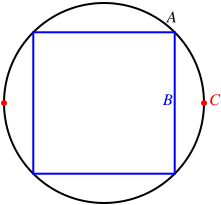
\includegraphics{HM_Example}}
\caption{Sets $A$, $B$, and $C$.}
\label{F:Hausdorff_Example}
\end{center}
\end{figure}

Determine $h(A,B)$, $h(A,C)$, and $h(B,C)$, and verify that $h(A,C) \leq h(A,B) + h(B,C)$. 
	
\item It may be surprising that $h$ as in Definition \ref{def:Hausdorff_distance} is actually a metric, but it is. The underlying space is the collection of nonempty compact subsets of $X$ which we denote at $\mathcal{H}(X)$. Prove the following theorem.

\begin{theorem} Let $X$ be a metric space. The Hausdorff distance function is a metric on $\mathcal{H}(X)$.
\end{theorem}

\item One fun application of the Hausdorff metric is in fractal geometry. You may be familiar with objects like the Sierpinski triangle or the Koch curve. These objects are limits of sequences of sets in $\mathcal{H}(\R^2)$. We illustrate with the Sierpinski triangle. Start with three points $v_1$, $v_2$, and $v_3$ that form the vertices of an equilateral triangle  $S_0$. For $i$=1,2, or 3, let $v_i = \begin{bmatrix} a_i \\ b_i \end{bmatrix}$. For $i$=1,2, or 3, we define $\omega_i : \R^2 \to \R^2$ by 
\[\omega_i\left(\begin{bmatrix} x \\ y \end{bmatrix}\right) = \begin{bmatrix} \frac{1}{2} & 0 \\ 0 & \frac{1}{2} \end{bmatrix}\begin{bmatrix} x \\ y \end{bmatrix} + \begin{bmatrix} a_i \\ b_i \end{bmatrix}.\]  
Then $\omega_i$, when applied to $S_0$, contracts $S_0$ by a factor of 2 and then translates the image of $S_0$ so that the $i^{\text{th}}$ vertex of $S_0$ and the $i$th vertex of the image of $S_0$ coincide. Such a map is called a \emph{contraction mapping} with \emph{contraction factor} equal to $\frac{1}{2}$.  Define $S_{1,i}$ to be $\omega_i(S_0)$. Then $S_{1,i}$  is the set of all points half way between any point in $S_0$  and  $v_i$, or $S_{1,i}$ is a triangle half the size of the original translated to the $i^{\text{th}}$ vertex of the original. Let $S_1 = \bigcup_{i=1}^3 S_{1,i}$. Both $S_0$ and $S_1$ are shown in figure \ref{F:Sierpinski}. We can continue this procedure replacing $S_0$ with $S_1$. In other words, for $i$ = 1, 2, and 3, let $S_{2,i} = \omega_i(S_1)$. Then let $S_2 = \bigcup_{i=1}^3 S_{2,i}$. A picture of $S_2$ is shown in figure \ref{F:Sierpinski}. We can continue this procedure, each time replacing $S_{j-1}$ with $S_j$. A picture of $S_8$ is shown in figure \ref{F:Sierpinski}.  

\begin{figure}[h]
\begin{center}
\begin{tabular}{cc}
\resizebox{!}{2.0in}{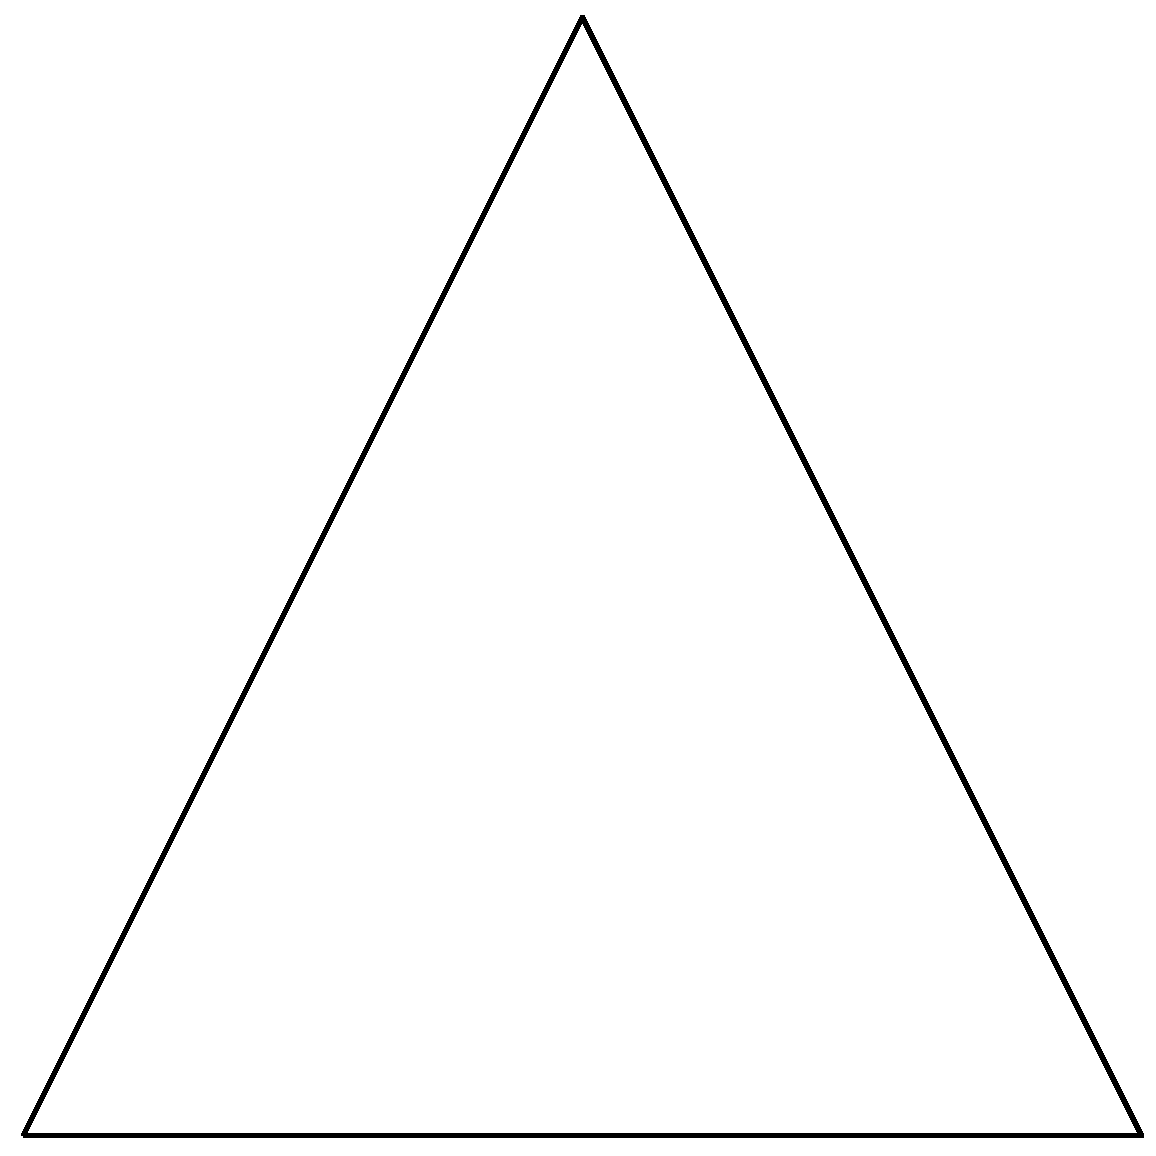
\includegraphics{S0.eps}}
&\resizebox{!}{2.0in}{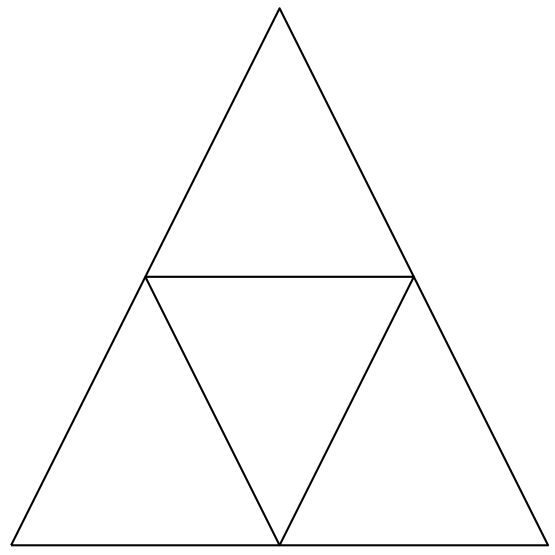
\includegraphics{S1.eps}} \\
$S_0$	&$S_1$ \\
\resizebox{!}{2.0in}{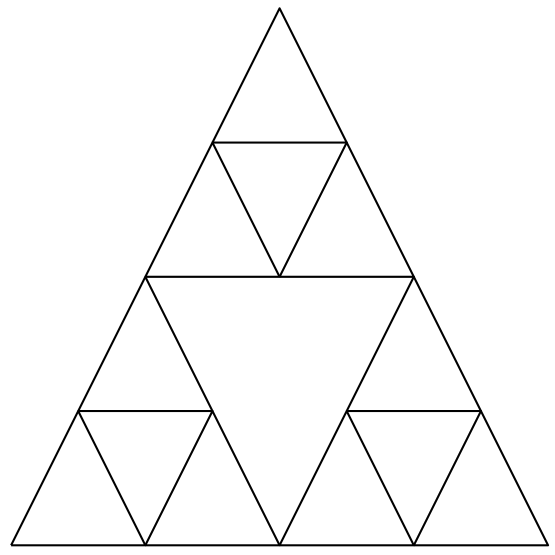
\includegraphics{S2.eps}}
&\resizebox{!}{2.0in}{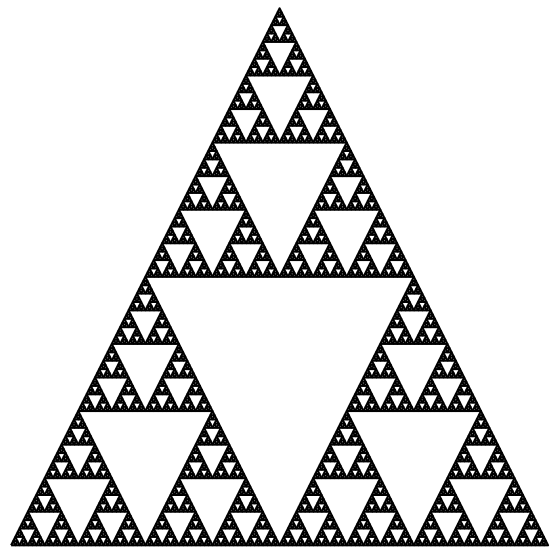
\includegraphics{S8.eps}} \\
$S_2$	&$S_8$ 
\end{tabular}
\caption{$S_i$ for $i$ equal to 0, 1, 2, and 8.}
\label{F:Sierpinski}
\end{center}
\end{figure}


To continue this process, we need to take a limit. But the $S_i$ are sets in $\mathcal{H}(\R^2)$, so the limit is taken with respect to the Hausdorff metric. 

	\begin{enumerate}[i.]
	
	\item Assume that the length of a side of $S_0$ is $1$. Determine $h(S_0,S_1)$. Then find $h(S_k, S_{k+1})$ for an arbitrary positive integer $k$. 
	
	\item The Sierpinski triangle will exist if the sequence $(S_n)$ converges to a set $S$ (which would be the Sierpinski triangle). The question of convergence is not a trivial one. 
	
		\begin{enumerate}[A.]
		
		\item Consider the sequence $(a_n)$, where $a_n = \left(1+\frac{1}{n}\right)^n$ for $n \in \Z^+$. Note that each $a_n$ is a rational number. Explain why the terms in this sequence get arbitrarily close together, but the sequence does not converge in $\Q$. Explain why the sequence $(a_n)$ converges in $\R$. 
		
	\item A sequence $(x_n)$ in a metric space $(X,d)$ is a \emph{Cauchy sequence}\index{Cauchy sequence} if given $\epsilon > 0$ there exists $N \in \Z^+$ such that $d(x_n, x_m) < \epsilon$ whenever $n, m \geq N$. Every convergent sequence is a Cauchy sequence. A metric space $X$ is said to be \emph{complete}\index{metric space!complete} if every Cauchy sequence in $X$ converges to an element in $X$. For example, $(\R, d_E)$ is complete while $(\Q, d_E)$ is not. Although we will not prove it, the metric space $(\mathcal{H}(\R^2), h)$ is complete. Show that the sequence $(S_n)$ is a Cauchy sequence in $\mathcal{H}(\R^2)$. The limit of this sequence is the famous Sierpinski triangle. The picture of $S_8$ in figure \ref{F:Sierpinski} is a close approximation of the Sierpinski triangle.
		
		\end{enumerate}
	
	\end{enumerate}

	\ea

\end{activity}

\begin{comment}

\ActivitySolution

\ba

\item Let $A = (0,1)$ and $B = (0,2)$ in $(\R,d_E)$. Then $d(A,B) = 0$ while $d(B,A) = d_E(2,1) = 1$.

\item Since $d(A,B) = d_E\left((0,1),\left(0, \frac{1}{\sqrt{2}}\right)\right) = \frac{1}{\sqrt{2}} = d(B,A)$, it follows that $h(A,B) = \frac{1}{\sqrt{2}}$. Now $d(C,A) = 0$ since $C \subset A$. However, $d(A,C) = d_E\left((0,1),(1,0)\right) = \sqrt{2}$. So $h(A,C) = \sqrt{2}$.  Since $d(C,B) = d_E\left((1,0), \left(\frac{1}{\sqrt{2}}, 0\right) \right) = 1-\frac{1}{\sqrt{2}}$ and $d(B,C) = d_E\left(\left(0, \frac{1}{\sqrt{2}}\right), (1,0)\right) = \frac{\sqrt{3}}{2}$, it follows that $h(B,C) = \frac{\sqrt{3}}{2}$. 

Then
\[h(A,C) = \sqrt{2} \leq \frac{\sqrt{2}}{2} + \frac{\sqrt{3}}{2} = h(A,B) + h(B,C).\]


\item  Let $X$ be a metric space and let $A$, $B$, and $C$ be in $\mathcal{H}(X)$. Since $d(A,B)$ is never negative, it follows that $h(A,B) \geq 0$. If $A \subseteq B$, then $d(a,B) = \min_{b \in B} \{d(a,B)\} = 0$ for every $a \in A$. So $d(A,A) = 0$. Also, if $h(A,B) = 0$, then both $d(A,B)$ and $d(B,A) = 0$. Since $d(A,B) = 0$, $\min_{b \in B} \{d(a,B)\}$ must be $0$ for every $a \in A$. But if $d(a,B) = 0$, the fact that $B$ is closed implies that $a \in B$. So $A \subseteq B$. Interchanging $A$ and $B$ shows that $B \subseteq A$ and $A  = B$. 

Finally, we verify the triangle inequality.  We know that either $h(A,C) = d(A,C)$ or $h(A,C) = d(C,A)$. Without loss of generality, assume $h(A,C) = d(A,C)$. Choose $a \in A$ such that $d(a,C) = d(A,C) = h(A,C)$. Now choose $c \in C$ such that $d_E(a,c) = d(a,C) = h(A,C)$.  

Let $b_a \in B$ and $c_a \in C$ such that $d_E(a,b_a) = d(a,B)$ and $d_E(b_a, c_a) = d(b_a,C)$. Since $d_E(a,c) = \min_{c' \in C} \{d_E(a,c')\}$, we know $d_E(a,c) \leq d_E(a,c_a)$. The triangle inequality for the metric $d$ gives us 
\[h(A,C) = d(A,C) = d_E(a,c) \leq d_E(a,c_a) \leq d_E(a,b_a) + d_E(b_a,c_a) = d(a,B) + d(b_a,C).\]
Since $d(a,B) \leq d(A,B)$ and $d(b_a,C) \leq d(B,C)$, we have 
\[h(A,C) \leq d(A,B) + d(B,C) \leq h(A,B) + h(A,C).\] 

	\begin{enumerate}[i.]
	
	\item Since $S_0 \subseteq S_1$, we have that $d(S_0,S_1) = 0$. The distance from $S_1$ to $S_0$ is the length of the line segment shown in Figure \ref{F:Sierpinski_2}. The length of the hypotenuse of the small triangle is $\frac{1}{4}$. By similar triangles, $d(S_1,S_0) = \frac{\sqrt{3}}{8} = h(S_0,S_1)$. Since the triangles shrink by a factor of $\frac{1}{2}$ every step, we can conclude that $h(S_k, S_{k+1}) = \frac{\sqrt{3}}{2^{k+3}}$ for $k \in \Z^+$. 
	\begin{figure}[h]
\begin{center}
\resizebox{!}{2.0in}{\includegraphics{dS1_S0.eps}}
\caption{$d(S_1,S_0)$.}
\label{F:Sierpinski_2}
\end{center}
\end{figure}
	
		\begin{enumerate}[A.]
		
		\item The sequence $(a_n)$ is a well-known sequence that converges to the real number $e$. Since the sequence $(a_n)$ converges in $\R$, the terms in this sequence get arbitrarily close together. However, because $e$ is not in $\Q$, the sequence $(a_n)$ does not converge in $\Q$.
				
	\item We know that $h(S_k, S_{k+1}) = \frac{\sqrt{3}}{2^{k+3}}$. Now, if $n$ and $m$ are positive integers with $n \leq m$ we have 
	\begin{align*}
	h(S_n,S_m) &\leq h(S_n, S_{n+1}) + h(S_{n+1}, S_{n+2}) + \cdots + h(S_{m-1}, S_{m}) \\
		&= \frac{\sqrt{3}}{2^{n+3}} + \frac{\sqrt{3}}{2^{n+4}} + \cdots + \frac{\sqrt{3}}{2^{m+2}} \\
		&= \frac{\sqrt{3}}{2^{n+3}}\left(1+\frac{1}{2} +  \cdots + \frac{1}{2^{m-n-1}}\right) \\
		&= \frac{\sqrt{3}}{2^{n+3}} \left(\frac{1 - \frac{1}{2^{m-n}}}{1-\frac{1}{2}} \right) \\
		&= \frac{\sqrt{3}}{2^{n+3}} \left(\frac{1 - \frac{1}{2^{m-n}}}{1-\frac{1}{2}} \right) \\
		&= \frac{\sqrt{3}}{2^{n+2}} \left(1 - \frac{1}{2^{m-n}}\right) \\
		&\leq  \frac{\sqrt{3}}{2^{n+2}}.
	\end{align*}
Let $\epsilon$ be a positive real number and choose $N$ such that $\frac{\sqrt{3}}{2^{N+2}} < \epsilon$. Then if $n,m < N$ with $n \leq m$ we have 
\[h(S_n,S_m) \leq \frac{\sqrt{3}}{2^{n+2}} \leq \frac{\sqrt{3}}{2^{N+2}} < \epsilon.\]
So $(S_n)$ is a Cauchy sequence. 
		
		\end{enumerate}
	
	\end{enumerate}


\ea

\end{comment}

